\documentclass[10pt,a4paper]{article}
\usepackage[utf8]{inputenc}
\usepackage[german]{babel}
\usepackage{amsmath}
\usepackage{amsfonts}
\usepackage{amssymb}
\usepackage{graphicx}
\usepackage[left=2cm,right=2cm,top=2cm,bottom=2cm]{geometry}

\begin{document}

\section*{Aufgabe 8.1}

\begin{tabular}{l|l|l|l|l}
a & b & c & r & s\\ \hline
0 & 0 & 0 & 0 & 0\\ \hline
0 & 0 & 1 & 0 & 1\\ \hline
0 & 1 & 0 & 0 & 1\\ \hline
0 & 1 & 1 & 1 & 0\\ \hline
1 & 0 & 0 & 0 & 1\\ \hline
1 & 0 & 1 & 1 & 0\\ \hline
1 & 1 & 0 & 1 & 0\\ \hline
1 & 1 & 1 & 1 & 1\\ \hline
\end{tabular}

\begin{equation}
r = \overline{a}bc + a\overline{b}c + ab\overline{c} + abc
\end{equation}
\begin{equation}
s = \overline{a}\overline{b}c + \overline{a}b\overline{c} + a\overline{b}\overline{c} + abc
\end{equation}

\section*{Aufgabe 8.2}

\begin{tabular}{l|l|l|l}
a & b & c & r\\ \hline
0 & 0 & 0 & 0\\ \hline
0 & 0 & 1 & 1\\ \hline
0 & 1 & 0 & 1\\ \hline
0 & 1 & 1 & 0\\ \hline
1 & 0 & 0 & 1\\ \hline
1 & 0 & 1 & 0\\ \hline
1 & 1 & 0 & 0\\ \hline
1 & 1 & 1 & 1\\ \hline
\end{tabular}

\begin{figure}[h]
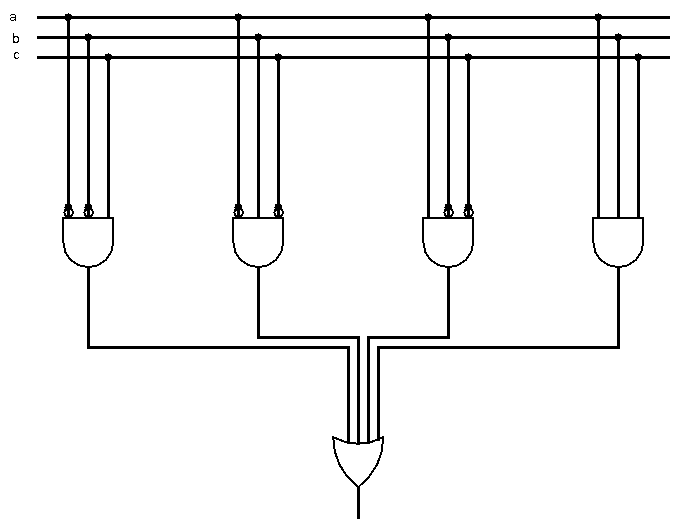
\includegraphics[scale=0.6]{8_2.png}
\end{figure}

\section*{Aufgabe 8.3}

\begin{equation}
r = \overline{a}b\overline{c} + \overline{a}bc + a\overline{b}c + abc
\end{equation}

\begin{figure}[h]
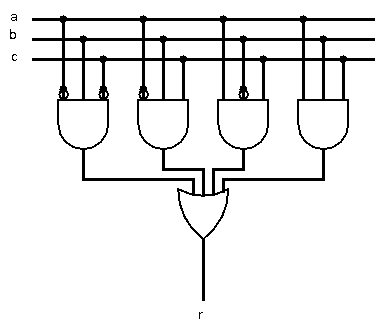
\includegraphics[scale=0.6]{8_3.png}
\end{figure}

\section*{Aufgabe 8.4}

\subsection*{Teil 1}

Da der Zusammenhang zwischen den Eingaben und Ausgaben nicht bekannt ist, kann keinerlei Zusammenhang angenommen werden.
Man kann auch keinerlei Zusammenhang herstellen, da jede mögliche Funktion in der Box implementiert sein könnte.
Es muss also jede Belegung einzeln getestet werden, was $3 \cdot 2^{5} = 96$ Messungen erfordert.

\subsection*{Teil 2}

Aus der Vorlesung wissen wir, dass eine Funktion mit $n$ Abhängigkeiten $2^{2^{n}}$ Funktionen implementieren kann.
Da wir hier 3 solche Funktionen haben, die beliebig zu einer Gesamtfunktion kombiniert werden können, könnten $(2^{2^{5}})^{3} = 2^{3 \cdot 2^{5}}$ Funktionen implementiert werden.

\section*{Aufgabe 8.5}

\begin{tabular}{l|l|l|l}
a & b & c & r\\ \hline
0 & 0 & 0 & 0\\ \hline
0 & 0 & 1 & 1\\ \hline
0 & 1 & 0 & 0\\ \hline
0 & 1 & 1 & 1\\ \hline
1 & 0 & 0 & 1\\ \hline
1 & 0 & 1 & 0\\ \hline
1 & 1 & 0 & 1\\ \hline
1 & 1 & 1 & 1\\ \hline
\end{tabular}

\subsection*{Teil 1}

\begin{equation}
DNF(r) = (a + b + c)(a + \overline{b} + c)(\overline{a} + b + \overline{c})
\end{equation}

\subsection*{Teil 2}

\begin{equation}
KNF(r) = \overline{a}\overline{b}c + \overline{a}bc + a\overline{b}\overline{c} + ab\overline{c} + abc
\end{equation}

\end{document}